\documentclass[10pt]{article}
\usepackage{../_macrosLatex/macros}
\usepackage[a4paper,margin=2.5cm]{geometry}
\usepackage{fancyhdr} % Gestion header/footer

%----------------------------------------------------
% Paramétrage de la fiche
%----------------------------------------------------
\matiere{BTS SNIR TS1}
\sequence{Programmation en langage C++}
\seqlogo{\faCode}
\titrefiche{C02 - Structures alternatives et répétitives}
\version{v1.0}
\dateversion{02.10.22}
\type{cours}
\repogithub{c02\_structuresAlternativesRepetitives}
\urlgithub{https://github.com/snir-ts1-cpp/c02\_structuresAlternativesRepetitives}

%----------------------------------------------------
% Définition des pieds et têtes de page
%----------------------------------------------------
% Pour toutes les pages
\pagestyle{fancy}
\fancyhead[L]{\seqlogo\ \sequenceVal}
\fancyhead[R]{\titreficheVal}
\fancyfoot[L]{\matiereVal - Lycée Louis Rascol, Albi}
\fancyfoot[R]{\ccbyncsaeu}
\fancyfoot[C]{\thepage\ / \pageref{LastPage}}
% Pour la première page
\fancypagestyle{firstpage}{%
    \lhead{}
    \rhead{}
    \renewcommand{\headrulewidth}{0pt}
}

%----------------------------------------------------
% Début du document
%----------------------------------------------------
\begin{document}
\renewcommand{\contentsname}{Sommaire} % Changement du nom de la table des matières
\cartouche
\thispagestyle{firstpage}

\introduction{assets/aiguillage.jpg}{Photo par \href{https://unsplash.com/@causeimluap}{causeimluap} sur \href{https://unsplash.com/}{unsplash}}{
    Dans ce cours, nous expliquons comment gérer le flux d'exécution d'un programme, nous découvrirons les structures alternatives
    et répétitives. 
    
    \smallskip
    Ces structures vont nous permettre respectivement de créer des programmes pouvant prendre une décision et exécuter des instructions en boucle suivant une condition donnée.\\
    Ces structures disponibles dans la majorité des langages de programmation, sont indispensables à l'implémentation d'algorithmes des plus
    simples aux plus évolués.
}

\licence

\github

\tableofcontents
\clearpage

%----------------------------------------------------
% Section 1
%----------------------------------------------------
\section{Les structures alternatives}
Les structures alternatives permettent d'exécuter un bloc de code dans certaines conditions et un autre bloc dans d'autres
conditions. Elles agissent comme un aiguilleur au niveau du flux d'exécution en le dirigeant dans telle ou telle direction
suivant la condition donnée.

%--------------------
% Structure if
%--------------------
\subsection{Structure Si : if}
La structure \mintinline{cpp}`if`  est faite pour exécuter une série d'instructions seulement quand une condition fixée est vraie.

\subsubsection{Définition d'une structure if}

\smallskip
\begin{wrapfigure}[10]{l}{\textwidth/2}
    \centering
    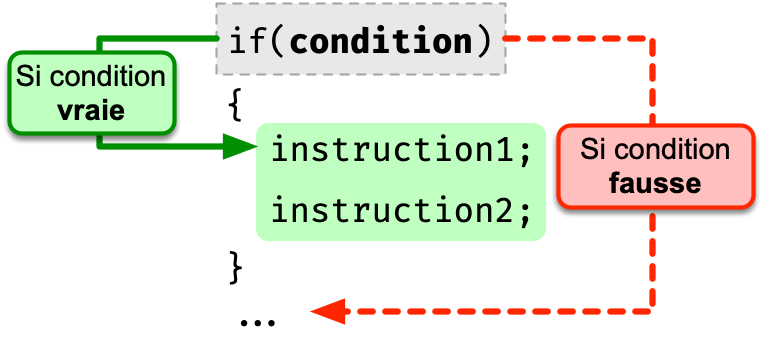
\includegraphics[max height=4cm,max width = \textwidth/2]{assets/if.jpg}
    \caption{Structure d'un \mintinline{cpp}`if`}
\end{wrapfigure}

Si la condition est \mintinline{cpp}`true` :
\begin{itemize}
    \item Les instructions présentes dans le corps du \mintinline{cpp}`if` sont \textbf{exécutées}.
    \item L'exécution continue sur la suite du code après le \mintinline{cpp}`if` 
\end{itemize}
Si la condition est \mintinline{cpp}`false` :
\begin{itemize}
    \item Les instructions présentes dans le corps du \mintinline{cpp}`if` sont \textbf{ignorées}
    \item L'exécution continue sur la suite du code après le \mintinline{cpp}`if` 
\end{itemize}

\subsubsection{Exemple 1 : Utilisation d'une structure if}

\cppfile{c02_structuresAlternativesRepetitives_projClion/sc1_structIf.cpp}
\captionof{listing}{Utilisation d'une structure \mintinline{cpp}`if`}
\label{exempleStrucIf}

\bigskip
Sortie console pour une saisie utilisateur d'un entier positif : \mintinline{cpp}`42`  :

\begin{textcode}
    Entrez un entier : 42
    Vous avez entre un entier positif : 42
    Cette ligne est toujours executee.
\end{textcode}

Sortie console pour une saisie utilisateur d'un entier négatif : \mintinline{cpp}`-81`  :

\begin{textcode}
    Entrez un entier : -81
    Cette ligne est toujours executee.
\end{textcode}

\etapesExec{
\begin{enumerate}
    \item Dans un premier temps, nous déclarons \mintinline{cpp}`nb`, variable qui va recevoir le nombre entier saisi par l'utilisateur \faArrowRight\ \textbf{l.7}.
    \item Nous nous occupons ensuite de l'affichage de la demande ainsi que de la lecture et du stockage de la saisie utilisateur dans la variable déclarée. \faArrowRight\ \textbf{l.8 et l.9}
    \item Puis, Nous mettons en œuvre une structure \mintinline{cpp}`if` dans laquelle la condition est sur l'entier \mintinline{cpp}`nb` : \mintinline{cpp}`nb > 0` \faArrowRight\ \textbf{l.11} 
    \begin{itemize}
        \item Si \mintinline{cpp}`nb` est strictement positif l'exécution sera aiguillée vers \faArrowRight\ \textbf{l.12} :\\
        \mintinline{cpp}`cout << "Vous avez entre un entier positif : " << number << endl;`\\
        Puis le flux d'exécution sortira de la structure \mintinline{cpp}`if` pour aller sur l'instruction suivante \faArrowRight\ \textbf{l.15} :\\
        \mintinline{cpp}`cout << "Cette ligne est toujours executee.";` 
        \item Si \mintinline{cpp}`nb` est négatif ou égal à 0 l'exécution sera aiguillée hors de la structure \mintinline{cpp}`if` vers l'instruction suivante \faArrowRight\ \textbf{l.15}  :\\
        \mintinline{cpp}`cout << "Cette ligne est toujours executee.";` 
    \end{itemize}
\end{enumerate}
}

%--------------------
% Structure if...else
%--------------------
\subsection{Structure Si Sinon : if...else}
La structure \mintinline{cpp}`if...else` est utilisée pour aiguiller le programme sur un bloc d'instructions dans le cas ou une condition fixée est juste et sur un autre bloc dans le cas ou la condition est fausse.

\subsubsection{Définition d'une structure if...else}

\smallskip
\begin{multicols}{2}
\begin{figure}[H]
    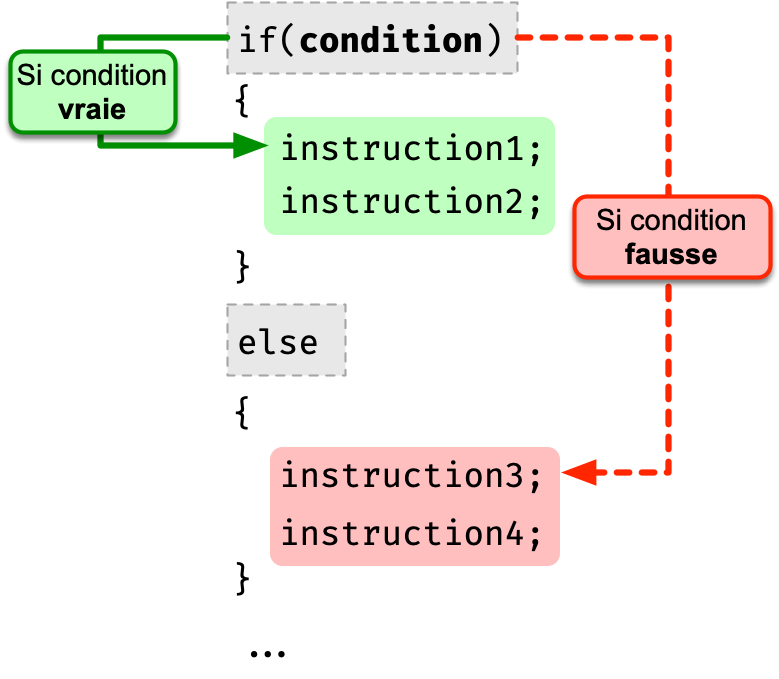
\includegraphics[max height=7cm,max width = \textwidth/2]{assets/ifElse.jpg}
    \centering
    \caption{Structure d'un \mintinline{cpp}`if...else`}
\end{figure}

Si la condition est \mintinline{cpp}`true` :
\begin{itemize}
    \item Les instructions présentes dans le corps du \mintinline{cpp}`if` sont \textbf{exécutées}.
    \item L'exécution continue sur la suite du code après le \mintinline{cpp}`if`
\end{itemize}
Si la condition est \mintinline{cpp}`false` :
\begin{itemize}
    \item Les instructions présentes dans le corps du \mintinline{cpp}`else` sont \textbf{exécutées}
    \item L'exécution continue sur la suite du code après le \mintinline{cpp}`if` 
\end{itemize}
\end{multicols}

\subsubsection{Exemple 2 : Utilisation d'une structure if...else}
\cppfile{c02_structuresAlternativesRepetitives_projClion/sc2_structIfElse.cpp}
\captionof{listing}{Utilisation d'une structure \mintinline{cpp}`if...else`}
\label{exempleStrucIfElse}

\bigskip
Sortie console pour une saisie utilisateur d'un entier positif : \mintinline{cpp}`42`  :

\begin{textcode}
    Entrez un entier : 42
    Vous avez entre un entier positif : 42
    Cette ligne est toujours executee.
\end{textcode}

Sortie console pour une saisie utilisateur d'un entier négatif : \mintinline{cpp}`-81`  :

\begin{textcode}
    Entrez un entier : -81
    Vous avez entre un entier negatif : -81
    Cette ligne est toujours executee.
\end{textcode}

\etapesExec{
\begin{enumerate}
    \item Dans un premier temps, nous déclarons \mintinline{cpp}`nb`, variable qui va recevoir le nombre entier saisi par l'utilisateur \faArrowRight\ \textbf{l.7}.
    \item Nous nous occupons ensuite de l'affichage de la demande ainsi que de la lecture et du stockage de la saisie utilisateur dans la variable déclarée. \faArrowRight\ \textbf{l.8 et l.9}
    \item Puis, nous mettons en œuvre une structure \mintinline{cpp}`if...else` dans laquelle la condition est sur l'entier \mintinline{cpp}`nb` : \mintinline{cpp}`nb >= 0` \faArrowRight\ \textbf{l.11}. 
    \begin{itemize}
        \item Si \mintinline{cpp}`nb` est positif ou égal à 0 l'exécution sera aiguillée vers les instructions dans le \mintinline{cpp}`if` \faArrowRight\ \textbf{l.12} :\\
         \mintinline{cpp}`cout << "Vous avez entre un entier positif : " << number << endl;`
        \item Sinon l'exécution sera aiguillée vers les instructions dans le \mintinline{cpp}`else` \faArrowRight\ \textbf{l.15} : \\
        \mintinline{cpp}`cout << "Vous avez entre un entier negatif: " << number << endl;` 
    \end{itemize}
    \item Une fois sorti de la structure \mintinline{cpp}`if` l'exécution du code continue et va sur l'instruction \faArrowRight\ \textbf{l.18} :\\
     \mintinline{cpp}`cout << "Cette ligne est toujours executee.";` 
\end{enumerate}
}

\begin{noteblock}
    \textbf{Utilisation des accolades \{ \}}
    
    \smallskip
    Dans le cas d'\textbf{une seule instruction} à exécuter dans le \mintinline{cpp}`if` ou dans le \mintinline{cpp}`else`, C++ nous autorise à ne pas mettre les accolades. Nous reprenons la structure du code source \ref{exempleStrucIfElse} sans accolades pour le \mintinline{cpp}`if...else` dans le code source \ref{ifElseSansAccolades}.
\end{noteblock}

\cppfile{c02_structuresAlternativesRepetitives_projClion/sc3_structIfElse_sansAccolades.cpp}
\captionof{listing}{Utilisation d'une structure \mintinline{cpp}`if...else` sans accolades}
\label{ifElseSansAccolades}

%----------------------
% Structure if..else if
%----------------------
\subsection{Structures Si imbriquées : if...else if}
La structure \mintinline{cpp}`if...else if` permet d'imbriquer les conditions suivies des blocs d'exécution les uns à la suite des autres.

\subsubsection{Définition d'une structure if...else if}

\smallskip
%Les étapes ci-dessous sont basées sur le diagramme de la figure \ref{structIfElseIf}

\begin{multicols}{2}
\begin{figure}[H]
    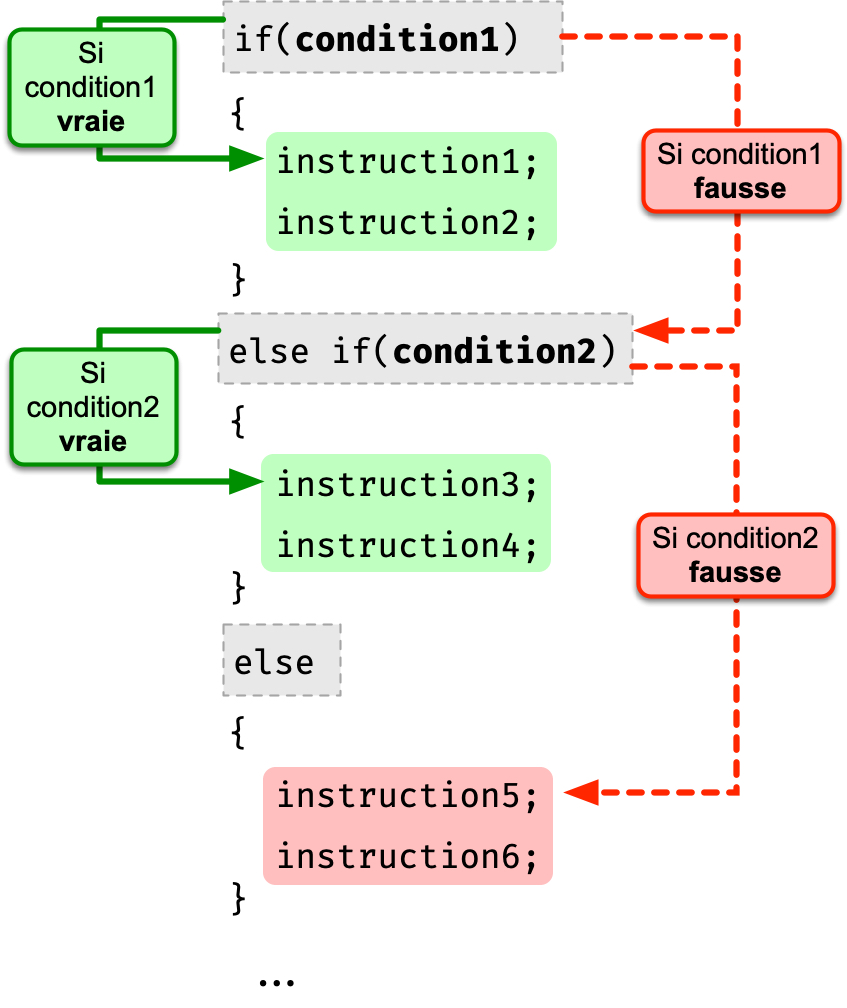
\includegraphics[max height=10cm,max width = \textwidth/2]{assets/ifElseIf.jpg}
    \centering
    \caption{Structure d'un \mintinline{cpp}`if...else if`}
    \label{structIfElseIf}
\end{figure}

\begin{itemize}
    \item Si \mintinline{cpp}`condition1` est \mintinline{cpp}`true`:\\  Le programme exécute les instructions 1 et 2 puis saute à la fin de la structure.
    \item Si \mintinline{cpp}`condition1` est \mintinline{cpp}`false`:\\ Le programme teste la deuxième condition \mintinline{cpp}`condition2` :
    \begin{itemize}
        \item Si \mintinline{cpp}`condition2` est \mintinline{cpp}`true`, le programme exécute les instructions 3 et 4 et saute à la fin de la structure.
        \item Si \mintinline{cpp}`condition2` est \mintinline{cpp}`false`, le programme exécute les instructions 4 et 5 du \mintinline{cpp}`else`. 
    \end{itemize}
\end{itemize}
\end{multicols}

\begin{noteblock}
    Nous ne sommes pas limité à un seul \mintinline{cpp}`else if` il est possible d'en ajouter autant que nécessaire entre le \mintinline{cpp}`if` et le \mintinline{cpp}`else`.
\end{noteblock}

\subsubsection{Exemple 3 : Utilisation d'une structure if...else if}

\cppfile{c02_structuresAlternativesRepetitives_projClion/sc4_structIfElseIf.cpp}
\captionof{listing}{Utilisation d'une structure \mintinline{cpp}`if...else`}
\label{exempleStrucIfElseIf}

\bigskip
Sortie console pour une saisie utilisateur d'un entier positif : \mintinline{cpp}`42`  :

\begin{textcode}
    Entrez un entier : 42
    Vous avez entre un entier positif : 42
    Cette ligne est toujours executee.
\end{textcode}

Sortie console pour une saisie utilisateur d'un entier négatif : \mintinline{cpp}`-81`  :

\begin{textcode}
    Entrez un entier : -81
    Vous avez entre un entier negatif : -81
    Cette ligne est toujours executee.
\end{textcode}

Sortie console pour une saisie utilisateur du nombre \mintinline{cpp}`0` :

\begin{textcode}
    Entrez un entier : 0
    Vous avez entre 0
    Cette ligne est toujours executee.
\end{textcode}

\etapesExec{
\begin{enumerate}
    \item Dans un premier temps, nous déclarons \mintinline{cpp}`nb`, variable qui va recevoir le nombre entier saisi par l'utilisateur \faArrowRight\ \textbf{l.7}.
    \item Nous nous occupons ensuite de l'affichage de la demande ainsi que de la lecture et du stockage de la saisie utilisateur dans la variable déclarée. \faArrowRight\ \textbf{l.8 et l.9}
    \item Puis, nous mettons en œuvre une structure \mintinline{cpp}`if...else if` \faArrowRight\ \textbf{l.11}:
    \begin{itemize}
        \item 1\up{ere} condition \mintinline{cpp}`nb > 0` \faArrowRight\ \textbf{l.11}:\\
        Si \mintinline{cpp}`nb` est positif le flux sera aiguillée vers les instructions dans le \mintinline{cpp}`if` :\\
        \mintinline{cpp}`cout << "Vous avez entre un entier positif : " << number << endl;`\\
        Sinon le flux d'exécution sera dirigé vers la seconde condition.
        \item 2\up{nd} condition \mintinline{cpp}`nb < 0` (\textbf{Uniquement si la 1ere est fausse}) \faArrowRight\ \textbf{l.14}:\\
        Si \mintinline{cpp}`nb` est négatif le flux sera aiguillé vers les instructions dans le \mintinline{cpp}`else if` :\\
        \mintinline{cpp}`cout << "Vous avez entre un entier negatif : " << nb << endl;`\\
        Sinon le flux d'exécution sera dirigé vers le \mintinline{cpp}`else`. 
        \item Instruction \mintinline{cpp}`else` \faArrowRight\ \textbf{l.17}: \\
        Si aucune des 2 conditions n'est \mintinline{cpp}`true`, l'instruction présente dans le \mintinline{cpp}`else` sera exécutée :\\
        \mintinline{cpp}`cout << "Vous avez entre 0"<< endl;` 
    \end{itemize}
    \item Une fois sorti de la structure \mintinline{cpp}`if` l'exécution du code continue et va sur l'instruction \faArrowRight\ \textbf{l.21}:\\
     \mintinline{cpp}`cout << "Cette ligne est toujours executee.";` 
\end{enumerate}
}

%------------------------
% Structure switch...case
%------------------------
\subsection{Structure Choix : switch...case}
La structure \mintinline{cpp}`switch...case` aiguille le flux d'exécution vers un bloc d'instruction suivant la valeur d'une variable donnée. Très utilisé dans l'implémentation de menus utilisateur, le \mintinline{cpp}`switch...case` permet de se passer de l'utilisation de plusieurs structures \mintinline{cpp}`if...else` imbriquées.

\subsubsection{Définition d'une structure switch...case}

\smallskip
\begin{multicols}{2}
\begin{figure}[H]
    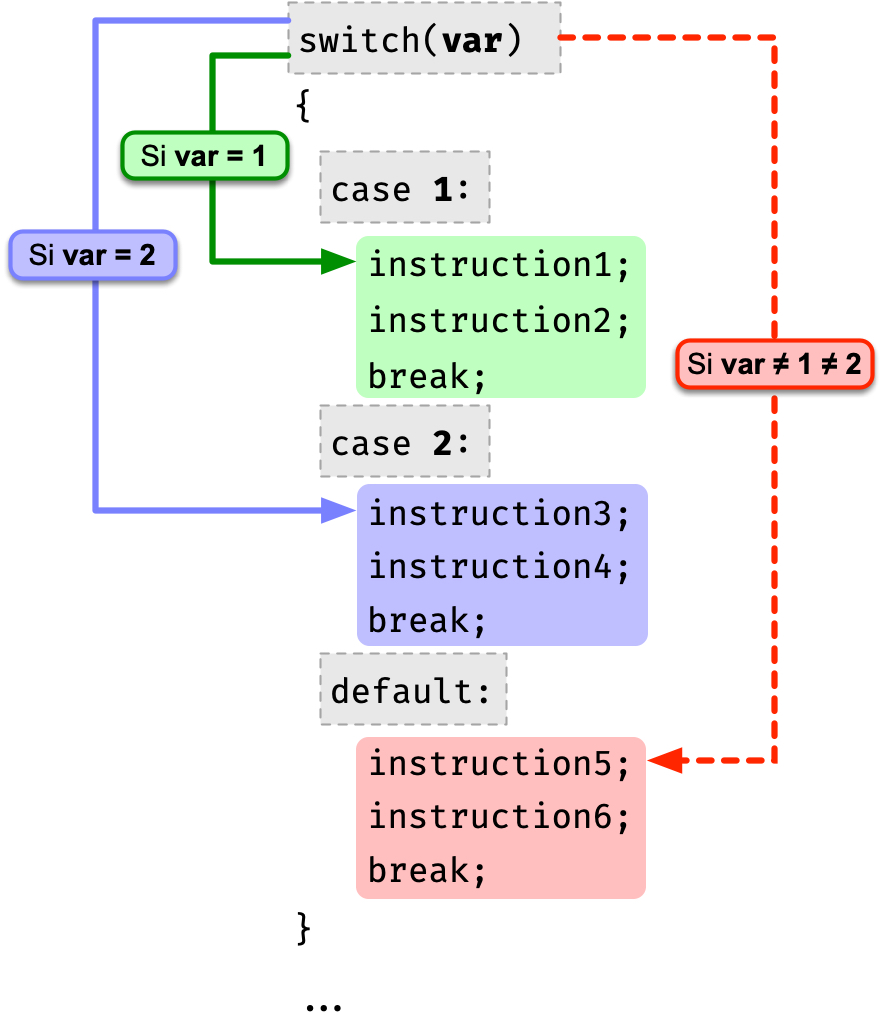
\includegraphics[max height=15cm,max width = \textwidth/2]{assets/switchCase.jpg}
    \centering
    \caption{Structure d'un \mintinline{cpp}`switch...case`}
\end{figure}

La variable autour duquel le choix va être fait s'apelle \mintinline{cpp}`var` :
\begin{itemize}
    \item Si \mintinline{cpp}`var` est égal à \mintinline{cpp}`1` alors le flux d'exécution sera dirigé vers le \mintinline{cpp}`case 1` et exécutera l'instruction 1 et 2.
    \item Si \mintinline{cpp}`var` est égal à \mintinline{cpp}`2` alors le flux d'exécution sera dirigé vers le \mintinline{cpp}`case 2` et exécutera l'instruction 3 et 4.
    \item Si \mintinline{cpp}`var` n'est ni égal à \mintinline{cpp}`1` ou a  \mintinline{cpp}`2` alors le flux d'exécution sera dirigé vers le \mintinline{cpp}`default` et exécutera l'instruction 5 et 6.
\end{itemize}
\end{multicols}

\subsubsection{Exemple 4 : Utilisation d'une structure switch...case}

\cppfile{c02_structuresAlternativesRepetitives_projClion/sc5_structSwitchCase.cpp}
\captionof{listing}{Utilisation d'une structure \mintinline{cpp}`switch...case`}

\bigskip
Sortie console pour une saisie utilisateur de \mintinline{text}`1` :

\begin{textcode}
    Entrez votre choix parmi 1, 2 ou 3 : 1
    Vous avez saisi 1
\end{textcode}

Sortie console pour une saisie utilisateur de \mintinline{text}`2` :

\begin{textcode}
    Entrez votre choix parmi 1, 2 ou 3 : 2
    Vous avez saisi 2
\end{textcode}

Sortie console pour une saisie utilisateur de \mintinline{text}`3` :

\begin{textcode}
    Entrez votre choix parmi 1, 2 ou 3 : 3
    Vous avez saisi 3
\end{textcode}

Sortie console pour une saisie utilisateur de \mintinline{text}`42` :

\begin{textcode}
    Entrez votre choix parmi 1, 2 ou 3 : 42
    Vous n'avez saisi ni 1, ni 2, ni 3
\end{textcode}

\etapesExec{
\begin{enumerate}
    \item Dans un premier temps nous déclarons la variable qui stockera le choix de l'utilisateur : \mintinline{cpp}`choixUtilisateur` \faArrowRight\ \textbf{l.7}
    \item Nous nous occupons ensuite de l'affichage de la demande et de lire et stocker la saisie utilisateur dans la variable déclarée. \faArrowRight\ \textbf{l.8 et l.9} 
    \item Puis, nous mettons en œuvre une structure \mintinline{cpp}`switch...case` avec pour variable de choix \mintinline{cpp}`choixUtilisateur` \faArrowRight\ \textbf{l.11}
    \item Suivant le contenu de la variable \mintinline{cpp}`choixUtilisateur`, le flux d'exécution sera aiguillé vers :
    \begin{itemize}
        \item \mintinline{cpp}`case 1` si le choix utilisateur est \mintinline{cpp}`1`, l'instruction \mintinline{cpp}`cout << "Vous avez saisi 1" << endl;` sera alors exécutée. \faArrowRight\ \textbf{l.14} 
        \item \mintinline{cpp}`case 2` si le choix utilisateur est \mintinline{cpp}`2`, l'instruction \mintinline{cpp}`cout << "Vous avez saisi 2" << endl;` sera alors exécutée. \faArrowRight\ \textbf{l.17} 
        \item \mintinline{cpp}`case 3` si le choix utilisateur est \mintinline{cpp}`3`, l'instruction \mintinline{cpp}`cout << "Vous avez saisi 3" << endl;` sera alors exécutée. \faArrowRight\ \textbf{l.20} 
        \item \mintinline{cpp}`default` si le choix utilisateur n'est ni \mintinline{cpp}`1`, ni \mintinline{cpp}`2`, ni \mintinline{cpp}`3`, l'instruction \mintinline{cpp}`cout << "Vous n'avez saisi ni 1, ni 2, ni 3" << endl;` sera alors exécutée. \faArrowRight\ \textbf{l.23} 
    \end{itemize}
    \item Le programme sort ensuite de la structure \mintinline{cpp}`switch...case` pour se terminer.
\end{enumerate}
}

\clearpage
%----------------------------------------------------
% Section 2
%----------------------------------------------------
\section{Les structures répétitives}

Les structures répétitives permettent de répéter un bloc d'instructions en boucle tant qu'une condition donnée est vraie.

%------------------------
% Structure while
%------------------------
\subsection{Boucle Tant que : while}
\subsubsection{Définition d'une structure while}

\smallskip
\begin{multicols}{2}
\begin{figure}[H]
    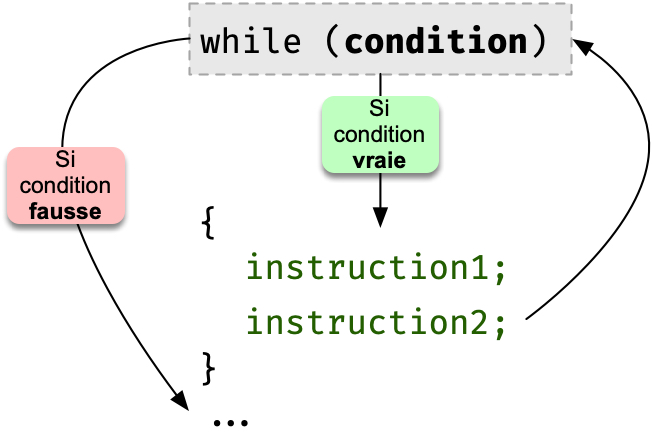
\includegraphics[max height=15cm,max width = \textwidth/2]{assets/while.jpg}
    \centering
    \caption{Structure d'un \mintinline{cpp}`while`}
\end{figure}

\begin{itemize}
    \item Les instructions 1 et 2 présentent dans le \mintinline{cpp}`while` seront exécutées en boucle \textbf{tant que la condition est vrai}.
    \item Si la condition est fausse, le flux d'exécution sortira de la structure.
    \item \textbf{La vérification de la condition est effectuée à chaque début de répétition}, dans le cas du diagramme avant d'exécuter \mintinline{cpp}`instruction1` et après avoir exécuté \mintinline{cpp}`instruction2` (dans le cas de la fin d'un tour de boucle).
\end{itemize}
\end{multicols}

\subsubsection{Exemple 1 : Utilisation d'une structure while}

\cppfile{c02_structuresAlternativesRepetitives_projClion/sc6_structWhile.cpp}
\captionof{listing}{Utilisation d'une structure \mintinline{cpp}`while`}

\bigskip
Sortie console pour le code précédent :

\begin{textcode}
    1 2 3 4 5
\end{textcode}

\etapesExec{
    \renewcommand{\arraystretch}{1.5}
    \centering
    \setlength\arrayrulewidth{.75pt}
    \begin{tabular}{|c|c|c|c|}
    \hline
    \textbf{\makecell{Passages}} & \textbf{\mintinline{cpp}`i`  avant le \mintinline{cpp}`while` } & \textbf{Test en début de \mintinline{cpp}`while` } & \textbf{\mintinline{cpp}`i`  après le \mintinline{cpp}`while`}\\ \hline
    1\up{er}      & \mintinline{cpp}`i = 1`  & \mintinline{cpp}`true`  &  \mintinline{cpp}`i = 2` \\ \hline
    2\up{nd}       & \mintinline{cpp}`i = 2`  & \mintinline{cpp}`true`  & \mintinline{cpp}`i = 3` \\ \hline
    3\up{eme}      & \mintinline{cpp}`i = 3`  & \mintinline{cpp}`true`  & \mintinline{cpp}`i = 4` \\ \hline
    4\up{eme}      & \mintinline{cpp}`i = 4`  & \mintinline{cpp}`true`  & \mintinline{cpp}`i = 5` \\ \hline
    5\up{eme}      & \mintinline{cpp}`i = 5`  & \mintinline{cpp}`true`  & \mintinline{cpp}`i = 6` \\ \hline
    6\up{eme}      & \mintinline{cpp}`i = 6`  & \mintinline{cpp}`false` &  \textbf{Pas d'exécution}\\ \hline
    \end{tabular}
}

\subsubsection{Boucle while infinie}

Dans certains cas, il peut être nécessaire de mettre en place une boucle \mintinline{cpp}`while`  infinie. Par exemple, le code C++ d'un système Arduino
doit fonctionner en boucle tant que la carte est sous tension, l'utilisation d'une boucle infinie est donc indispensable.

\cppfile{c02_structuresAlternativesRepetitives_projClion/sc7_structWhileInfinie.cpp}
\captionof{listing}{Exemple de structure \mintinline{cpp}`while` infinie}

Sortie console :

\begin{textcode}
    0 1 2 3 4 5 6 7 8 9 10 11 12 13 14 15 16 17 18 19 20 21 22 23 24 25 ...
\end{textcode}

\etapesExec{
    Dans le code ci-dessus, nous mettons en place une structure \mintinline{cpp}`while` avec pour condition \mintinline{cpp}`1`, cela signifie
    que la condition est toujours \mintinline{cpp}`true` donc les instructions dans la structure s'exécuteront sans fin.
    
    \smallskip
    Ici la variable \mintinline{cpp}`i` initialisée à \mintinline{cpp}`O` s'incrémente de 1 à chaque tour de boucle après avoir été affichée à l'écran.
}


%------------------------
% Structure do...while
%------------------------
\subsection{Boucle Faire Tant que : do...while}
\subsubsection{Définition d'une structure do...while}

\smallskip
\begin{multicols}{2}
\begin{figure}[H]
    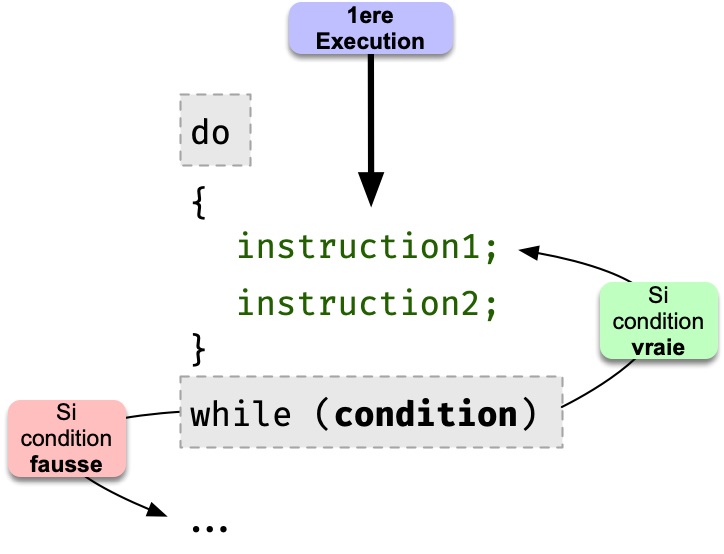
\includegraphics[max height=15cm,max width = \textwidth/2]{assets/do...while.jpg}
    \centering
    \caption{Structure d'un \mintinline{cpp}`do...while`}
\end{figure}

\begin{itemize}
    \item Dès que le flux d'exécution arrive sur la structure \mintinline{cpp}`do...while` \textbf{les instructions 1 et 2 sont exécutées une première fois sans que la condition soit vérifiée}.
    \item Après l'exécution des instructions, la condition est vérifiée :
    \begin{itemize}
        \item Si la condition est vraie, les instructions sont exécutées une nouvelle fois.
        \item Si la condition est fausse, le flux d'exécution sort de la structure \mintinline{cpp}`do...while`.
    \end{itemize}
\end{itemize}
\end{multicols}

\subsubsection{Exemple 2 : Utilisation d'une structure do...while}

\cppfile{c02_structuresAlternativesRepetitives_projClion/sc8_structDoWhile.cpp}
\captionof{listing}{Utilisation d'une structure \mintinline{cpp}`do...while`}

\bigskip
Sortie console pour le code précédent :

\begin{textcode}
    1 2 3 4 5
\end{textcode}

\etapesExec{
    \renewcommand{\arraystretch}{1.5}
    \centering
    \setlength\arrayrulewidth{.75pt}
    \begin{tabular}{|c|c|c|c|}
    \hline
    \textbf{\makecell{Passages}} & \textbf{\makecell{\mintinline{cpp}`i` avant le bloc\\ d'instructions}} & \textbf{\makecell{\mintinline{cpp}`i`  après le bloc\\ d'instructions}} & \textbf{\makecell{Test en fin \\de bloc}}\\ \hline
    1\up{er}      & \mintinline{cpp}`i = 1`  & \mintinline{cpp}`i=2`& \mintinline{cpp}`true` \\ \hline
    2\up{nd}       & \mintinline{cpp}`i = 2` & \mintinline{cpp}`i=3` & \mintinline{cpp}`true`\\ \hline
    3\up{eme}      & \mintinline{cpp}`i = 3` & \mintinline{cpp}`i=4` & \mintinline{cpp}`true`\\ \hline
    4\up{eme}      & \mintinline{cpp}`i = 4` & \mintinline{cpp}`i=5` & \mintinline{cpp}`true`\\ \hline
    5\up{eme}      & \mintinline{cpp}`i = 5` & \mintinline{cpp}`i=6` & \mintinline{cpp}`false`\\ \hline
    \end{tabular}
}

\begin{noteblock}
    \textbf{Comparaison \mintinline{cpp}`while` / \mintinline{cpp}`do...while`}
    
    \smallskip 
    Pour comparer cette structure avec la précédente, vous remarquerez que le programme à fait 5 tests sur la valeur de \mintinline{cpp}`i` pour le \mintinline{cpp}`do...while` et 6 tests pour le \mintinline{cpp}`while` cela est dû à la position du test dans chaque structure : au début pour le \mintinline{cpp}`while` et à la fin pour le \mintinline{cpp}`do...while`.
    
    \smallskip
    Pour cette dernière, le bloc d'instructions de la structure s'exécutera alors au moins une fois avant que la condition soit vérifiée.
\end{noteblock}

%------------------------
% Structure for
%------------------------
\subsection{Boucle Pour : for}

\subsubsection{Définition d'une structure for}

\smallskip
\begin{figure}[H]
    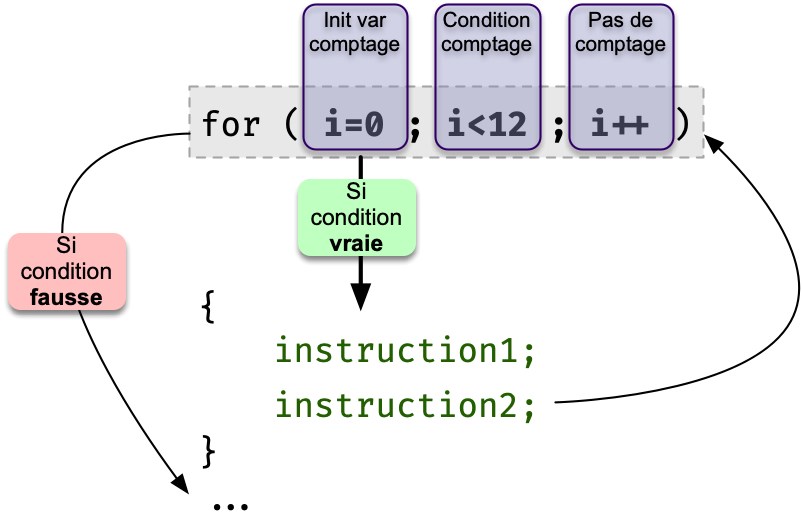
\includegraphics[max height=15cm,max width = 10cm]{assets/for.jpg}
    \centering
    \caption{Structure d'un \mintinline{cpp}`for`}
\end{figure}

\begin{itemize}
    \item La structure \mintinline{cpp}`for` \textbf{définit au début le nombre de fois où les instructions seront exécutées}.
    \item Nous devons saisir en argument du \mintinline{cpp}`for` : 
    \begin{itemize}
        \item \textbf{La variable de comptage initialisée} : Où je commence à compter ?
        \item \textbf{La condition de comptage} : Je compte tant que quoi ?
        \item \textbf{Le pas de comptage} : Je compte de combien en combien ?
    \end{itemize}
    \item Les instructions 1 et 2 présentent dans le \mintinline{cpp}`for` seront exécutées en boucle \textbf{tant que la condition de comptage est vrai}.
    \item Si la condition est fausse, le flux d'exécution sortira de la structure.
    \item \textbf{La vérification de la condition est effectuée à chaque début de répétition}, dans le cas du diagramme avant d'exécuter \mintinline{cpp}`instruction1` et après avoir exécuté \mintinline{cpp}`instruction2` (dans le cas de la fin d'un tour de boucle).
\end{itemize}

\subsubsection{Exemple 3 : Utilisation d'une structure for}

\cppfile{c02_structuresAlternativesRepetitives_projClion/sc9_structFor.cpp}
\captionof{listing}{Utilisation d'une structure \mintinline{cpp}`for`}

\bigskip
Sortie console pour le code précédent :

\begin{textcode}
    1 2 3 4 5
\end{textcode}

\etapesExec{
    Dans une boucle \mintinline{cpp}`for` le flux d'exécution parcours les étapes suivantes :\\
    \textbf{Exécution du bloc d'instruction \faAngleRight\ Incrément de la variable de comptage \faAngleRight\ Test sur la condition}

    \medskip
    \renewcommand{\arraystretch}{1.5}
    \begin{center}
        \setlength\arrayrulewidth{.75pt}
        \begin{tabular}{|c|c|c|c|}
        \hline
        \textbf{\makecell{Passages}} & \textbf{Affichage de \mintinline{cpp}`i`  } & \textbf{Incrément \mintinline{cpp}`i++`  } & \textbf{Test \mintinline{cpp}`i <= 5` }\\ \hline
        1\up{er}      & \mintinline{cpp}`1`  & \mintinline{cpp}`1+1=2`  &  \mintinline{cpp}`2<=5 == true` \\ \hline
        2\up{nd}       & \mintinline{cpp}`2`  & \mintinline{cpp}`2+1=3`  & \mintinline{cpp}`3<=5 == true` \\ \hline
        3\up{eme}      & \mintinline{cpp}`3`  & \mintinline{cpp}`3+1=4`  & \mintinline{cpp}`4<=5 == true` \\ \hline
        4\up{eme}      & \mintinline{cpp}`4`  & \mintinline{cpp}`4+1=5`  & \mintinline{cpp}`5<=5 == true` \\ \hline
        5\up{eme}      & \mintinline{cpp}`5`  & \mintinline{cpp}`5+1=6`  & \mintinline{cpp}`6<=5 == false` \\ \hline
        6\up{eme}      & \textbf{Pas d'exécution}  &  &  \\ \hline
        \end{tabular}    
    \end{center}
}

\subsection{Quand utiliser une structure while ou for ?}

Pour un même problème, les 3 structures expliquées précédemment permettent de faire la même chose : répéter un bloc d'instruction un certain nombre de fois. 
Seule l'implémentation sera différente et certaines structures se prêteront mieux à d'autres pour un problème donné. Nous donnons une règle générale à respecter
ci-dessous.

\important{Règle d'utilisation d'un \mintinline{cpp}`for` ou d'un \mintinline{cpp}`while`}{
    \begin{itemize}
        \item \textbf{Je connais le nombre de fois} où je vais devoir tourner dans la boucle : J'utilise une \textbf{boucle \mintinline{cpp}`for`}
        \item \textbf{Je ne connais pas le nombre de fois} où je vais tourner dans la boucle : J'utilise une \textbf{boucle \mintinline{cpp}`while` ou \mintinline{cpp}`do...while`} 
    \end{itemize}
}

\end{document}  